 
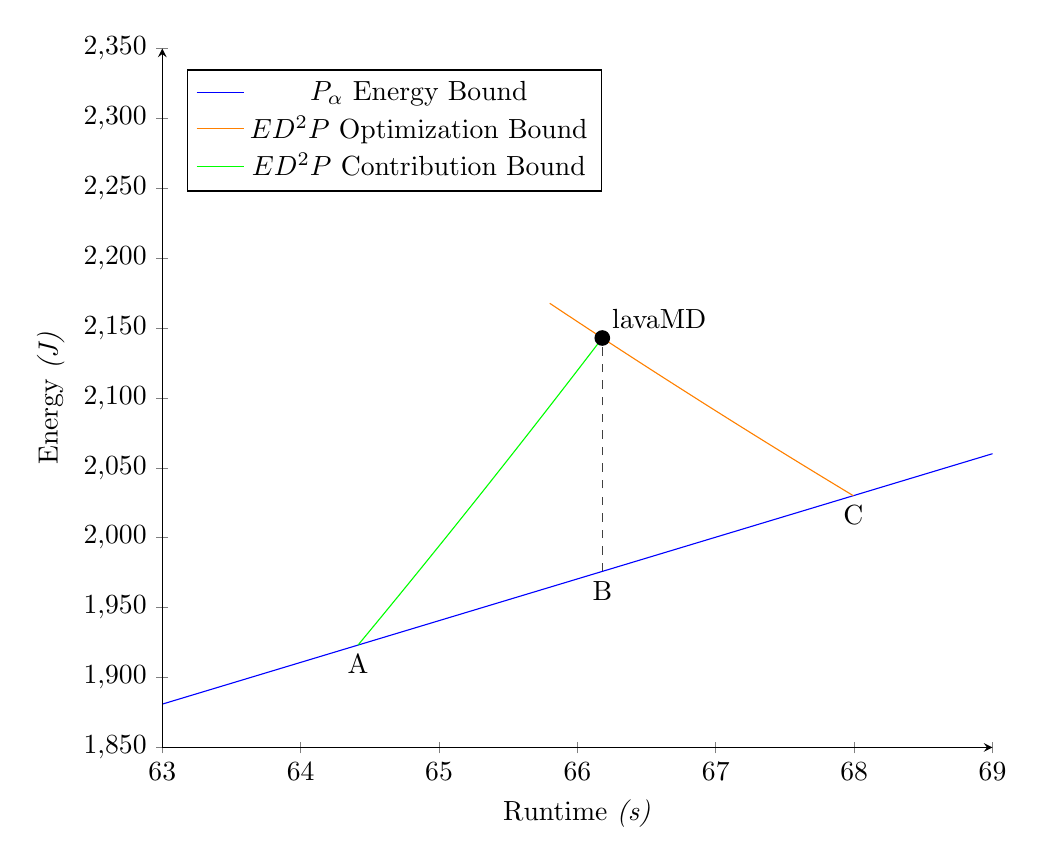
\begin{tikzpicture}
  \begin{axis}[    axis x line=bottom,axis y line=left,
ylabel={Energy \emph{(J)}}, xlabel={Runtime \emph{(s)}}, axis on top,
    xmin=63, xmax=69,
    ymin=1850, ymax=2350,
    width=\linewidth,
    legend style={legend pos=north west}
    ]

    %% Model Parameters %%
    \pgfmathsetmacro{\baselinepower}{29.857} % NOP code, 4 cores, 3.2 ghz
    \pgfmathsetmacro{\codepower}{32.38}
    \pgfmathsetmacro{\codetime}{66.18}
    % Sadly, pgfplots sucks too much to calculate cube roots
    \pgfmathsetmacro{\anodex}{64.4144}
    \pgfmathsetmacro{\anodey}{\anodex * \baselinepower}
    \pgfmathsetmacro{\cnodex}{67.994}
    \pgfmathsetmacro{\cnodey}{\cnodex * \baselinepower}
    \pgfmathsetmacro{\tnodex}{65.8}

    %% Intermezzo Values %%
    \pgfmathsetmacro{\codeenergy}{\codepower * \codetime}
    \pgfmathsetmacro{\baselineenergy}{\baselinepower * \codetime}
    \pgfmathsetmacro{\lowdisplayline}{(2 * \baselinepower + \codepower) / 3}

    % arguments: code power, code time, x - todo, apparently not supposed to do pgfmathparse
    \pgfmathdeclarefunction{metricbound}{3}{%
      \pgfmathparse{((#1 * #2^3) / #3^2)}%
    }
    \pgfmathdeclarefunction{definitionbound}{3}{%
      \pgfmathparse{((#1 / #2^3) * #3^4)}%
    }
     \pgfmathdeclarefunction{optimizationlimits}{3}{%
      \pgfmathparse{(min(metricbound(#1, #2, #3), definitionbound(#1, #2, #3)))}
    }

    % ALPHA BASELINE BOUND 
    \addplot[domain=\pgfkeysvalueof{/pgfplots/xmin}:\pgfkeysvalueof{/pgfplots/xmax},
             blue] {\baselinepower * x};
    \addlegendentry{$P_{\alpha}$ Energy Bound} 
    % BETA ROOFLINE BOUND

    % Constant Time and Power Dashes
    \draw[darkgray, dashed] ({axis cs:\codetime,\baselineenergy}) -- ({axis cs:\codetime,\codeenergy});
 

    \addplot[domain=\tnodex:\cnodex, orange] { metricbound(\codepower, \codetime, x)};
    \addlegendentry{$ED^{2}P$ Optimization Bound}
%
    \addplot[domain=\anodex:\codetime, green] { definitionbound(\codepower, \codetime, x)};
    \addlegendentry{$ED^{2}P$ Contribution Bound}


    \node[circle,fill,inner sep=2pt] at (axis cs:\codetime,\codeenergy) {};
    \node[above right] at (axis cs:\codetime,\codeenergy) {lavaMD};
    
    \node [below] at ({axis cs:\anodex, \anodey}) {A};
    \node [below] at ({axis cs:\codetime,\baselineenergy}) {B};
    \node [below] at ({axis cs:\cnodex, \cnodey}) {C};


 \end{axis}
\end{tikzpicture}
